\documentclass{article}
\textwidth=6in
\hoffset=0in
\voffset=0in

\usepackage{dcolumn}
\usepackage{afterpage}
\usepackage{pgf}
\usepackage{tikz}
\usepackage{pdflscape}
\usetikzlibrary{arrows,automata}
\usepackage[latin1]{inputenc}
\usepackage{ngerman}
\usepackage[a4paper, total={6in, 8in}]{geometry}
\usepackage{amsmath}
\usepackage{amssymb}
\usepackage{stmaryrd}
\usepackage{graphicx}
\usepackage{tikz}
\usetikzlibrary{automata, arrows, fit, calc}
\usepackage{pifont}
\usepackage{amssymb}
\usepackage{gensymb}
\usepackage[ampersand]{easylist}


\usepackage{listings}

\newcommand{\gap}{\ \\ \\}

\setcounter{section}{2}

% needs to be updated
\author{Max Springenberg, 177792}
\title{SWK\\
       "Ubungsblatt 2\\
       Gruppe 2: OH12 / 1.056}
\setcounter{section}{2}


\begin{document}

\subsection{}
\subsection{}
\subsection{git}

\subsubsection\ 
(i)\\
Mit \# gekennzeichnete lines bezeichnen Kommentare.\\
Das Editieren der Datei, musste nicht angegeben werden, deshalb ist es 
    auskommentiert.\\
\begin{verbatim}
    # S1:
    $ git init
    # touch data.txt
    $ git add data.txt
    $ git commit -m "first commit"
    # S2:
    $ git checkout -b fork
    # S3:
    # echo f > data.txt
    $ git  add data.txt
    $ git commit -m "fork commit"
    $ git checkout master
    # echo m > data.tx
    $ git add data.txt
    $ git commit -m "master commit"
    # S4:
    $ git merge fork
    # An dieser stelle werden wir auf einen merge-conflict aufmerksam gemacht
    $ git mergetool
    $ git commit -m "resolved merge-conflict"
\end{verbatim}
\gap
(ii)\\
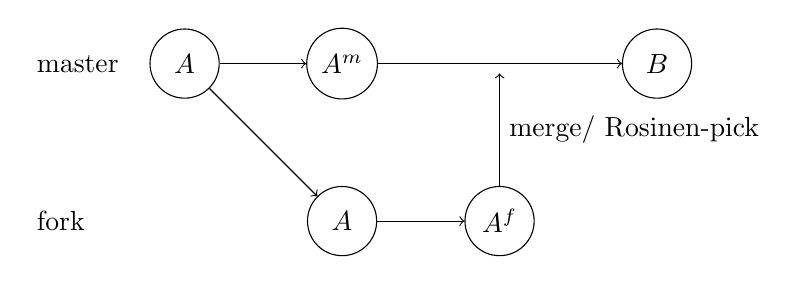
\begin{tikzpicture}
    \node[anchor=west] (master) at (0,0) {master};
    \node[anchor=west] (fork) at (0,-2) {fork};

    \node[state] (am) at (2,0) {$A$};
    \node[state] (af) at (4,-2) {$A$};
    \node[state] (a'f) at (6,-2) {$A^{f}$};
    \node[state] (a'm) at (4,0) {$A^{m}$};

    \node[state] (b) at (8,0) {$B$};
    \node[] (mpoint) at (6,0) {};

    \path 
        (am) 
            edge [->] node {} (af)
            edge [->] node {} (a'm)
        (af)
            edge [->] node {} (a'f)
        (a'm)
            edge [->] node {} (b)
        (a'f)
            edge [->, right] node {merge/ Rosinen-pick} (mpoint)
    ;
\end{tikzpicture}

\end{document}
